\chapter{Evaluierung}\label{chap:evaluation}

  \section{Evaluation der gesetzten Ziele}\label{sec:evaluation-goals}
    \subsection{Evaluation der Must-Haves}\label{subsec:evaluation-must-haves}
      Die detaillierte Analyse in Abschnitt \ref{subsec:impl-medusa-summary} verdeutlicht, dass die zentralen Anforderungen an das System erfolgreich umgesetzt wurden.
      Das Softwaremodul \ac{medusa} ist in der Lage, nicht-planare Pfade innerhalb des im Projekt abgesteckten Rahmens zuverlässig und mathematisch korrekt zu berechnen.

      Die Implementierung der Dateischnittstelle für \ac{STL}-Daten, welche sowohl das \ac{ASCII}- als auch das Binärformat unterstützt, erfüllt die in Abschnitt \ref{subsec:prioritization-and-evaluation-logic} definierten Zielvorgaben vollumfänglich.
      Wie in Abschnitt \ref{subsubsec:impl-medusa-mesh-import} dargelegt, gewährleistet die Integration der Assimp-Bibliothek hierbei eine robuste Datenverarbeitung.

      Entsprechend der Erläuterungen in Abschnitt \ref{subsec:impl-medusa-ui} und der Darstellung in Abbildung \ref{fig:T-planar} erfolgt die Visualisierung der geplanten Werkzeugpfade innerhalb von \ac{medusa} fehlerfrei.
      Diese grafische Rückkopplung ermöglicht eine unmittelbare Validierung der berechneten Trajektorien vor der Ausführung.
      \sig{Ben Stahl}

      \begin{figure}[H]
      \centering
      \includegraphics[width=0.3\textwidth]{dependencies/pictures/tplanar.png}
      \caption{Visualisierung des \texttt{T}-Modells innerhalb von \ac{medusa}, inklusive der generierten Trajektorien und der Pfadplanung.}
      \label{fig:T-planar}
      \end{figure}

    \subsection{Evaluation der Should-Haves}\label{subsec:evaluation-should-haves}
      Ein als „Should-Have“ klassifiziertes Ziel stellte die Pfadplanung für komplexe Geometrien mit 90\degree-Überhängen dar.
      Diese Funktionalität konnte erfolgreich implementiert werden und arbeitet, wie in Abbildung \ref{fig:T-planar} dokumentiert, ohne Einschränkungen.
      \sig{Ben Stahl}

    \subsection{Evaluation der Could-Haves}\label{subsec:evaluation-could-haves}
      Im Zuge der Anforderungsanalyse in Abschnitt \ref{subsec:prioritization-and-evaluation-logic} wurden neben den Kernfunktionalitäten zudem optionale Zielsetzungen identifiziert, um den Funktionsumfang des Systems zu erweitern.
      Besonders hervorzuheben ist hierbei die erfolgreiche Erweiterung der unterstützten Dateischnittstellen. Über das obligatorische \ac{STL}-Format hinaus bietet das System nun, wie in Abschnitt \ref{subsubsec:concept-medusa-pipeline} erwähnt, eine Unterstützung für das \ac{OBJ}-Format.
      Diese zusätzliche Dateikompatibilität steigert die Flexibilität des Slicers erheblich, da komplexe Geometriedaten nun aus einer breiteren Palette von \ac{CAD}- und Modellierungssoftware direkt importiert werden können.

      Ein weiteres erfolgreich realisiertes und als „Could-Have“ definiertes Entwicklungsziel betrifft die Interaktivität der grafischen Benutzeroberfläche.
      Es wurde eine funktionale Erweiterung in die \ac{GUI} von \ac{medusa} integriert, welche es dem Anwender erlaubt, prozesskritische Parameter wie die Schichtdicke dynamisch und intuitiv anzupassen.
      Durch diese Implementierung entfällt die Notwendigkeit, Modifikationen direkt im Quellcode vornehmen zu müssen, was die Benutzerfreundlichkeit sowie die Effizienz bei der iterativen Prozessoptimierung signifikant steigert.
      \sig{Ben Stahl}

    \subsection{Evaluation der Won’t-Haves}\label{subsec:evaluation-wont-haves}
      Bewusst ausgeschlossene Funktionalitäten wurden im Rahmen der Entwicklung konsequent nicht berücksichtigt.
      Dementsprechend erfolgt keine Ansteuerung realer Hardware zur Materialextrusion, weshalb auch keine physischen Bauteile gefertigt wurden.
      Zudem verfügt das System über keine Logik zur automatisierten Erkennung oder Reparatur defekter \ac{STL}-Netze, welche nicht den in Abschnitt \ref{subsec:prioritization-and-evaluation-logic} definierten Spezifikationen entsprechen.
      Es wird daher für den Prozessverlauf vorausgesetzt, dass die bereitgestellten \ac{STL}-Daten den qualitativen Mindestanforderungen genügen.
      \sig{Ben Stahl}


  \section{Evaluation der entwickelten Slicing-Algorithmen} \label{sec:evaluation-of-slicing-algorithms}
    Im Verlauf dieses Projektes wurden insgesamt eine Multiachs, sowie zwei differenzierte nicht planare Slicing-Strategien konzipiert und ausgearbeitet.
    Diese Strategien sowie deren theoretische Fundamente werden im Abschnitt \ref{sec:concept-of-slicing-strategies} detailliert definiert und gegenübergestellt.

    \subsection{Evaluation des Base-Slicing-Algorithmus}\label{subsec:evaluation-of-base-slicer}
      Der in Abschnitt \ref{subsec:concept-base-algorithm} beschriebene Base-Algorithmus, welcher im Rahmen dieser Studienarbeit entwickelt wurde, erfüllt die Kriterien eines Multiaxis Slicing Verfahrens gemäß den in Abschnitt \ref{subsec:planar-and-non-planar-slicing} beschriebenen Anforderungen.
      Die softwaretechnische Umsetzung dieses Verfahrens ist in Abschnitt \ref{subsubsec:impl-base-algorithm} umfassend dokumentiert.
      Aufgrund seiner inhärenten Fähigkeit zur mehrachsigen Schichtgenerierung diente dieser Algorithmus als essenzielle Grundlage für die weiterführende Entwicklung spezialisierter, nicht-planarer Slicing-Verfahren.
      Die erfolgreiche Implementierung dieses Basis-Algorithmus ist in Abbildung \ref{fig:T-planar} zu sehen, welche die Visualisierung der generierten Trajektorien und die Pfadplanung für das \texttt{T}-Modell zeigt.
      \sig{Ben Stahl}

    \subsection{Evaluation der sphärenbasierten Strategie}\label{subsec:evaluation-of-sphere-slicer}
      Die erste im Projektverlauf untersuchte nicht-planare Strategie ist die in Abschnitt \ref{subsec:concept-sphere-algorithm} dargelegte Sphären-Strategie.
      Dieses Konzept nutzt das Prinzip sich konzentrisch vergrößernder Sphären, um eine erhöhte strukturelle Stabilität des Bauteils zu generieren.
      Es stellte sich jedoch heraus, dass bei der Initialisierung einer neuen Sphäre an einem Überhang kritische Diskontinuitäten entstehen können, welche potenzielle mechanische Schwachstellen im Bauteilgefüge darstellen.
      Aufgrund dieser systemischen Defizite wurde von einer finalen Implementierung dieser Strategie abgesehen.
      Gleichwohl lieferte dieser Ansatz wichtige Erkenntnisse für die nachfolgende, optimierte Variation, welche die genannten Schwachpunkte erfolgreich adressiert und schließlich implementiert wurde.
      \sig{Ben Stahl}

    \subsection{Evaluation der kristallbasierten Strategie}\label{subsec:evaluation-of-crystal-slicer}
      Wie in Abschnitt \ref{subsec:concept-crystal-algorithm} detailliert ausgeführt, repräsentiert der Kristall-Algorithmus eine synergetische Verbindung aus dem sphärenbasierten Ansatz und der Basisstrategie für flächennormale Schichtung.
      Dieses Verfahren ermöglicht eine hochkomplexe, nicht-planare Toolpath-Planung, die mittels einer „Look Ahead“-Funktion Überhänge frühzeitig identifiziert und die Schichtgeometrie durch eine entsprechende Krümmung adaptiv anpasst.
      Durch diese fließenden Übergänge wird die strukturelle Integrität, insbesondere in kritischen Überhangbereichen, signifikant gesteigert.
      Die Implementierung dieses Algorithmus wird in \ref{subsubsec:impl-crystal-algorithm} dargelegt und stellt als leistungsfähigste Strategie zur Erzeugung nicht-planarer Schichten das zentrale Ergebnis dieses Projektes dar.
      Dieser Algorithmus ist in der Lage, eine präzise und zuverlässige Toolpath-Generierung durchzuführen, welche die nachfolgende Abbildungen~\ref{fig:T-nichtplanar} sowie \ref{fig:pyramide} darstellt.
      \sig{Ben Stahl}

  \section{Evaluation der Anforderungen an \acs{medusa}} \label{sec:evaluation-of-medusa-requirements}
    Das Softwaresystem \ac{medusa} erfüllt vollumfänglich die spezifizierten Anforderungen an einen nicht-planaren Slicer, wie bereits in Abschnitt \ref{sec:implementation-of-component-medusa} dargelegt wurde.
    Darüber hinaus verfügt das System über eine Referenzimplementierung eines planaren Slicers, die als Validierungsgrundlage für konventionelle Fertigungsstrategien dient.
    Ergänzend dazu wurde, wie in Abschnitt \ref{subsubsec:impl-crystal-algorithm} näher erläutert, ein spezialisierter Algorithmus für das nicht-planare Slicing erfolgreich implementiert.
    Dieser Algorithmus ist in der Lage, eine präzise und zuverlässige Toolpath-Generierung durchzuführen, welche die nachfolgende Abbildung~\ref{fig:T-nichtplanar} darstellt.

    Ein weiterer zentraler Aspekt ist die prozesssichere Verarbeitung von Geometriedaten im \ac{STL}-Format.
    Das Einlesen dieser Dateien, welches in Abschnitt \ref{subsec:prioritization-and-evaluation-logic} als kritisches Entwicklungsziel definiert wurde, funktioniert nun uneingeschränkt und fehlerfrei.
    Die technische Realisierung dieser Schnittstelle basiert auf der Integration der Assimp-Bibliothek, deren Implementierungsdetails umfassend in Abschnitt \ref{subsubsec:impl-medusa-mesh-import} dokumentiert sind.
    \sig{Ben Stahl}

  \section{Evaluation der Anforderungen an \acs{kronos}} \label{sec:evaluation-of-kronos-requirements}
    Das Teilsystem \ac{kronos} erfüllt zum gegenwärtigen Entwicklungsstand bereits den Großteil der in Abschnitt \ref{subsec:kronos-requirements} spezifizierten Anforderungen.
    Insbesondere ist \ac{kronos} in der Lage, diskrete Datenpunkte erfolgreich aus \ac{JSON}-Dateien zu extrahieren und diese als Grundlage für komplexe, weiterführende Berechnungen zu nutzen.
    Ein aktueller Limitationspunkt besteht jedoch darin, dass die Übergabe der generierten \ac{JSON}-Dateien an das System derzeit noch manuell erfolgen muss und noch nicht in einen vollautomatisierten Workflow integriert ist.
    Dies war jedoch auch nicht als Anforderung definiert.

    Die algorithmische Überführung der Datenpunkte in steuerungsrelevante Informationen ist grundsätzlich funktional, weist jedoch in spezifischen Fällen noch Optimierungspotenzial auf.
    So wurde beobachtet, dass der Inverse-Kinematik-Solver unter bestimmten mathematischen Randbedingungen keinen validen Toolpath generieren kann, was zu einer Unterbrechung der Trajektorienberechnung führt.
    Zudem tritt vereinzelt das Phänomen auf, dass der resultierende Toolpath zwischen zwei definierten Wegpunkten keine Linearität aufweist.
    Diese Abweichungen im Bewegungsverhalten müssen in künftigen Iterationen durch eine Verfeinerung des Solvers sowie eine optimierte Interpolationslogik adressiert werden.
    
    In der folgenden Abbildung~\ref{fig:toolpathKronos} ist die Doppelpyramide in \ac{kronos} dargestellt, welche die Visualisierung des abgefahrenen Toolpaths zeigt.
    Dies veranschaulicht die erfolgreiche Berechnung der Bewegungsabläufe sowie die funktionale Integration der Trajektorien in die Simulationsumgebung von \ac{kronos}.
    
    \begin{figure}[H]
    \centering
    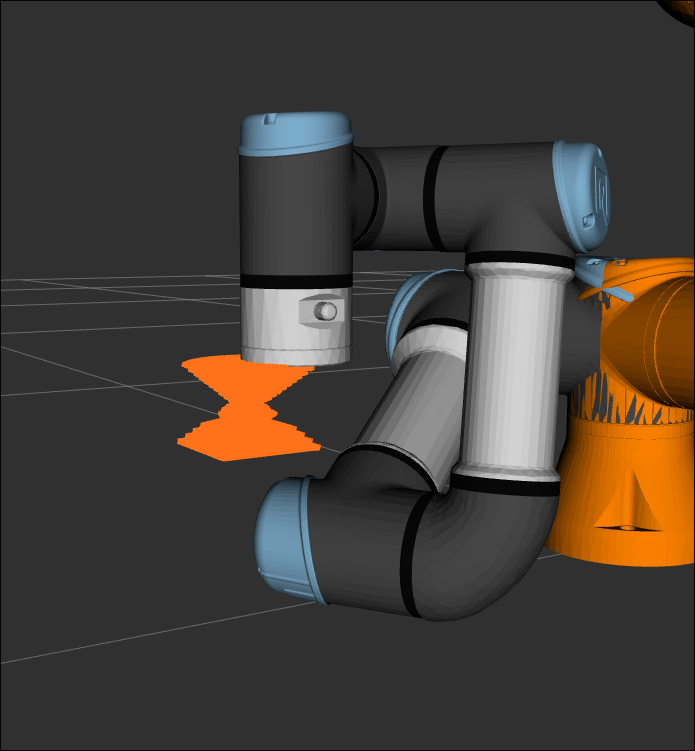
\includegraphics[width=0.4\textwidth]{dependencies/pictures/toolpathKronos.png}
    \caption{Screenshot der Doppelpyramide in \ac{kronos}, mitsamt des abgefahrenen Toolpaths.}
    \label{fig:toolpathKronos}
    \end{figure}
    \sig{Ben Stahl}

  \section{Versuchsaufbau}\label{sec:experimental-setup}
    Im Rahmen der vorliegenden Arbeit ist es erfolgreich gelungen, eine vollumfänglich simulierte Testumgebung zu projektieren und zu implementieren.
    Diese Entwicklungsumgebung basiert auf dem Framework \ac{ROS} 2 in Kombination mit MoveIt 2 sowie dem Visualisierungstool RViz, um das kinematische Verhalten des virtuellen Universal Robots UR3e realitätsgetreu abzubilden.
    Zu sehen ist die simulierte Umgebung in Abbildung~\ref{fig:simulation-environment-rviz}, welche die Darstellung des UR3e-Roboterarms sowie die Visualisierung des Druckbetts zeigt.

    \begin{figure}[H]
    \centering
    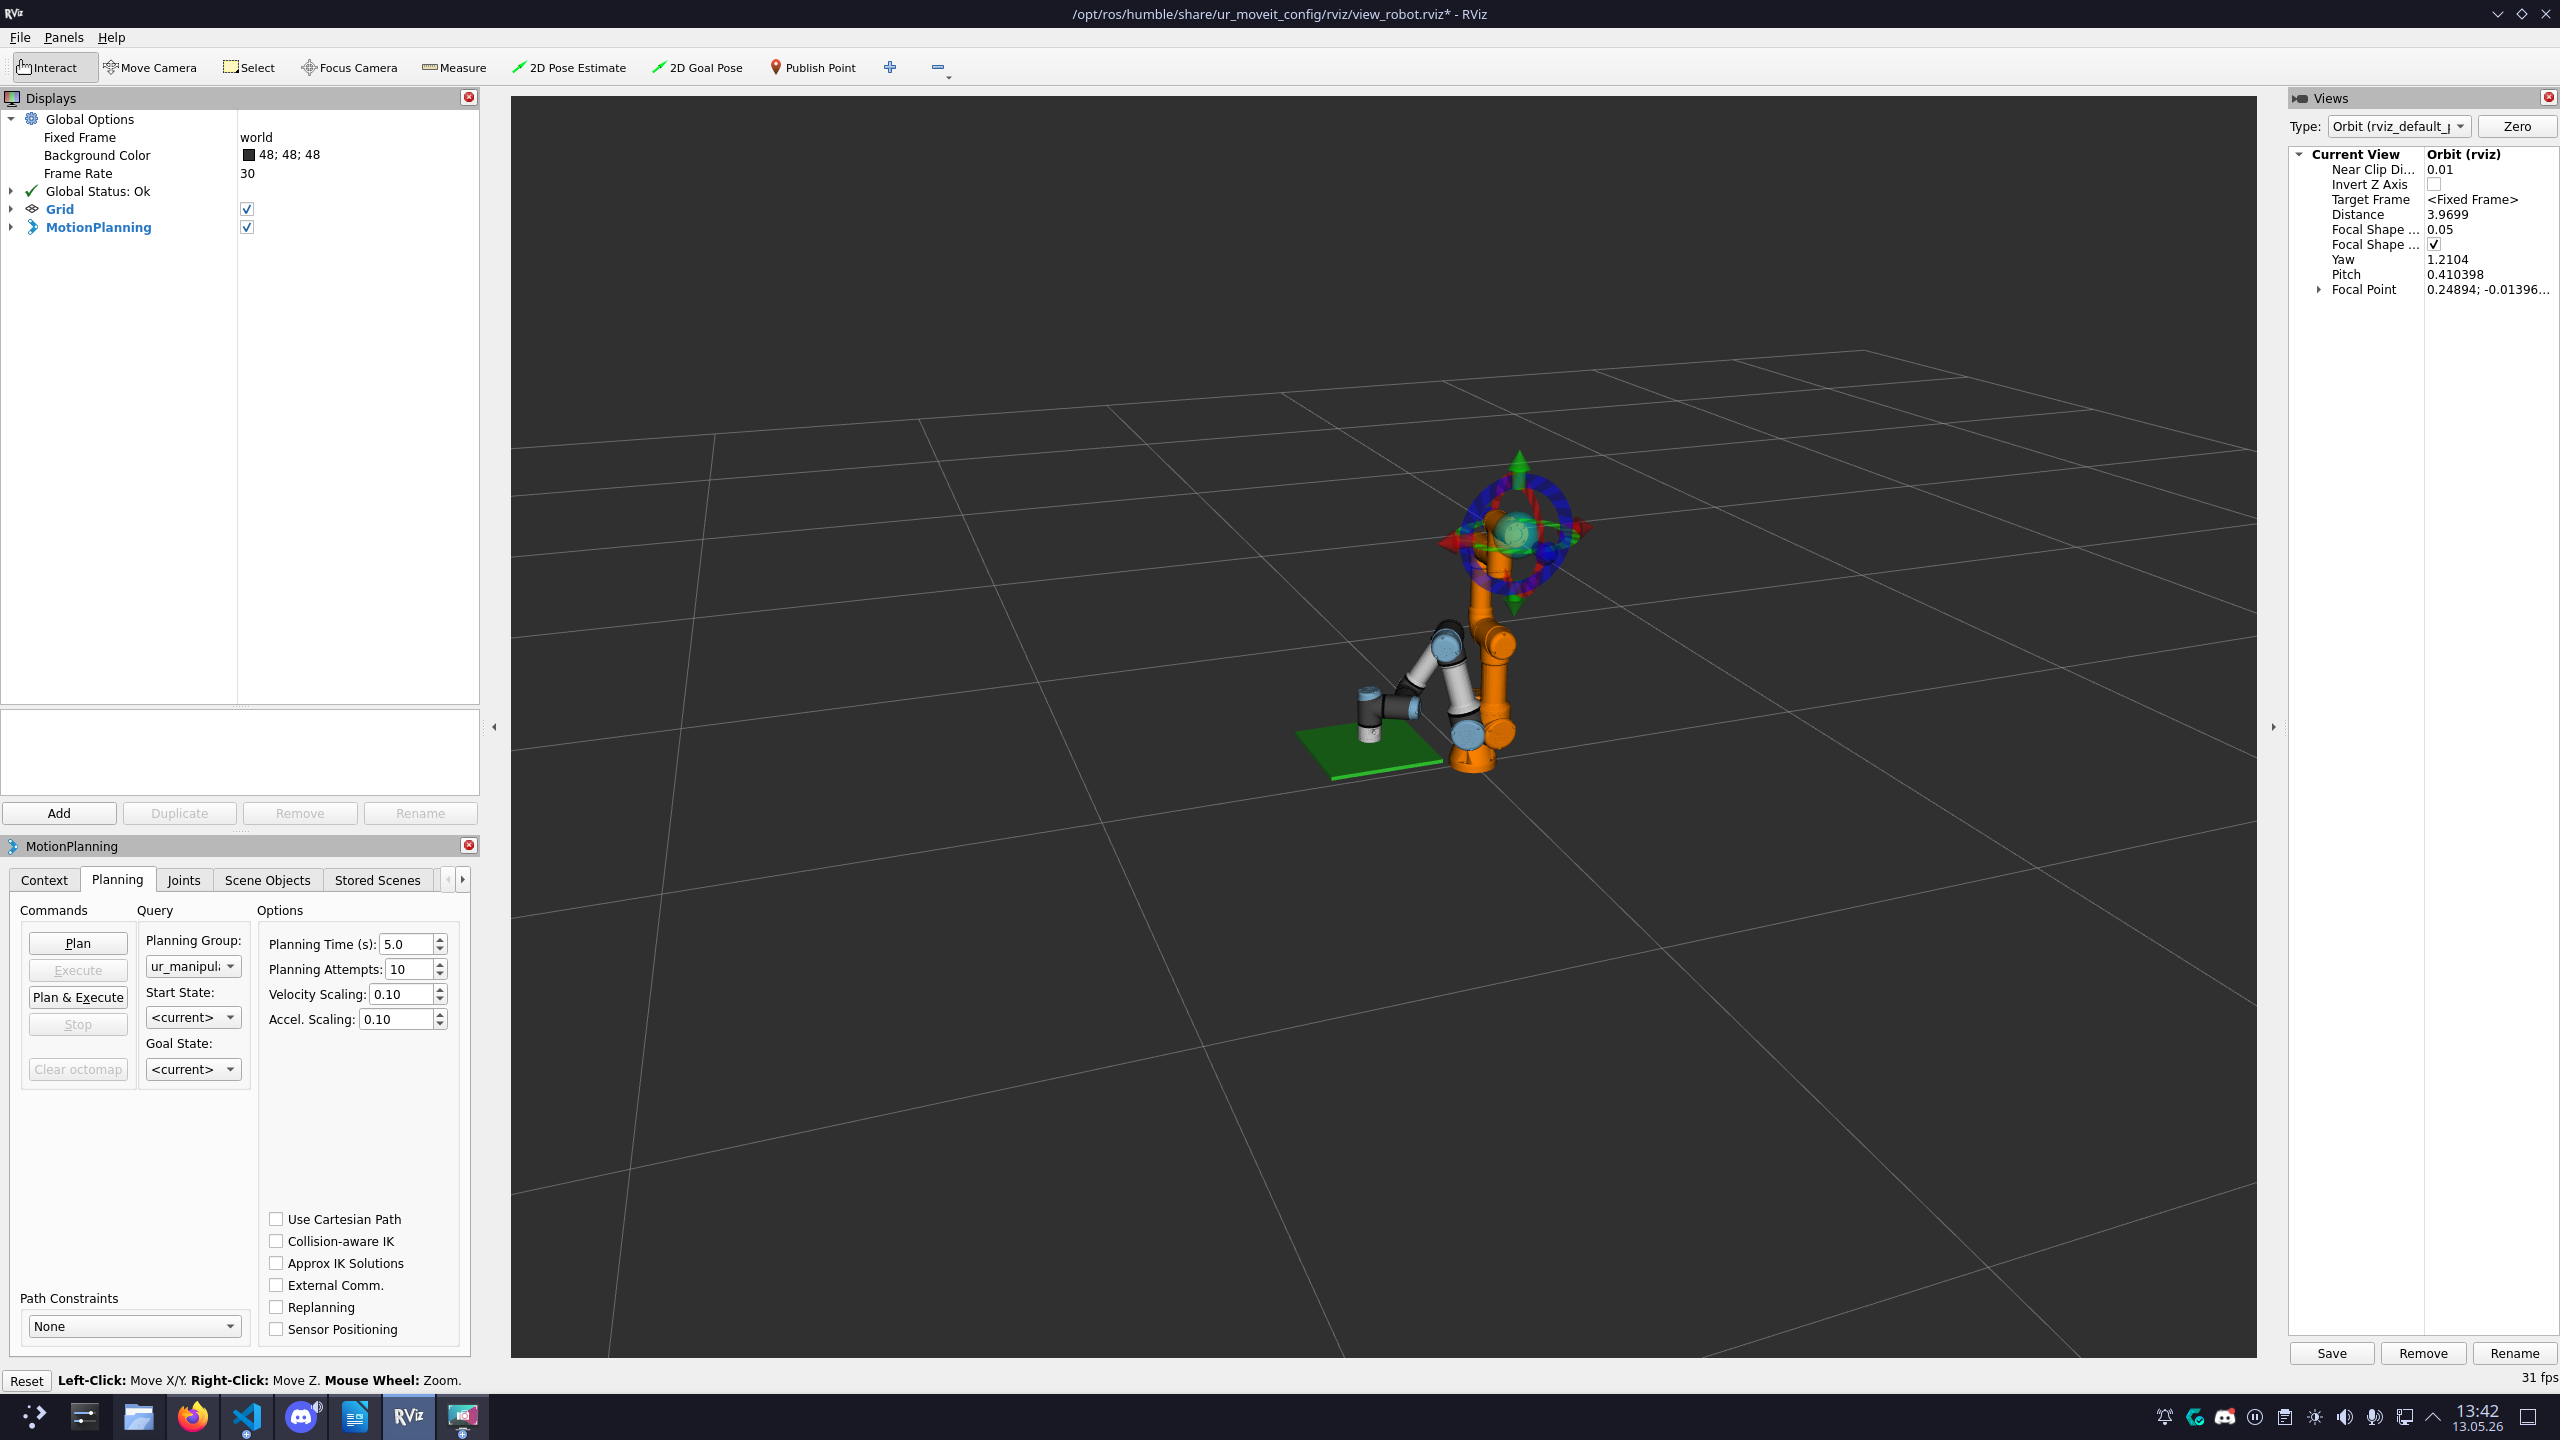
\includegraphics[width=0.6\textwidth]{dependencies/pictures/RVIs_simulation.png}
    \caption{Screenshot der Simulationsumgebung in RViz, welche die Darstellung des UR3e-Roboterarms sowie die Visualisierung Druckbretts zeigt.}
    \label{fig:simulation-environment-rviz}
    \end{figure}

    Zur Validierung des entwickelten Slicing-Verfahrens und der Bewegungssteuerung wurden drei spezifische \ac{STL}-Modelle als Referenzgeometrien herangezogen.
    Zunächst fungiert ein klassischer Würfel als Basismodell zur Überprüfung der grundlegenden Maßhaltigkeit und Schichtgenerierung.
    Darauf aufbauend wurde eine Doppelpyramide implementiert, anhand derer analysiert werden kann, wie der Slicing-Algorithmus mit moderaten Überhängen sowie kontinuierlichen Querschnittsveränderungen, namentlich Verkleinerungen und Vergrößerungen der Schichtflächen, interagiert.
    Den Abschluss der Testreihe bildet ein komplexes \texttt{T}-Modell, welches gezielt dazu dient, die Handhabung von kritischen 90\degree-Überhängen innerhalb der additiven Fertigungsstrategie zu demonstrieren.

    In den begleitenden Abbildungen ist die erfolgreiche Generierung der Trajektorien sowie das funktionale Pathplanning visualisiert.
    Der Abbildung~\ref{fig:pyramide} ist die Doppelpyramide in \ac{medusa} zu entnehmen, welche die generierten Trajektorien und die Visualisierung des Pathplannings illustriert.
    Das \texttt{T}-Modell ist in Abbildung~\ref{fig:T-nichtplanar} dargestellt, ebenfalls mitsamt der generierten Trajektorien und der Visualisierung des Pathplannings.
    \sig{Ben Stahl}

    \begin{figure}[H]
    \centering
    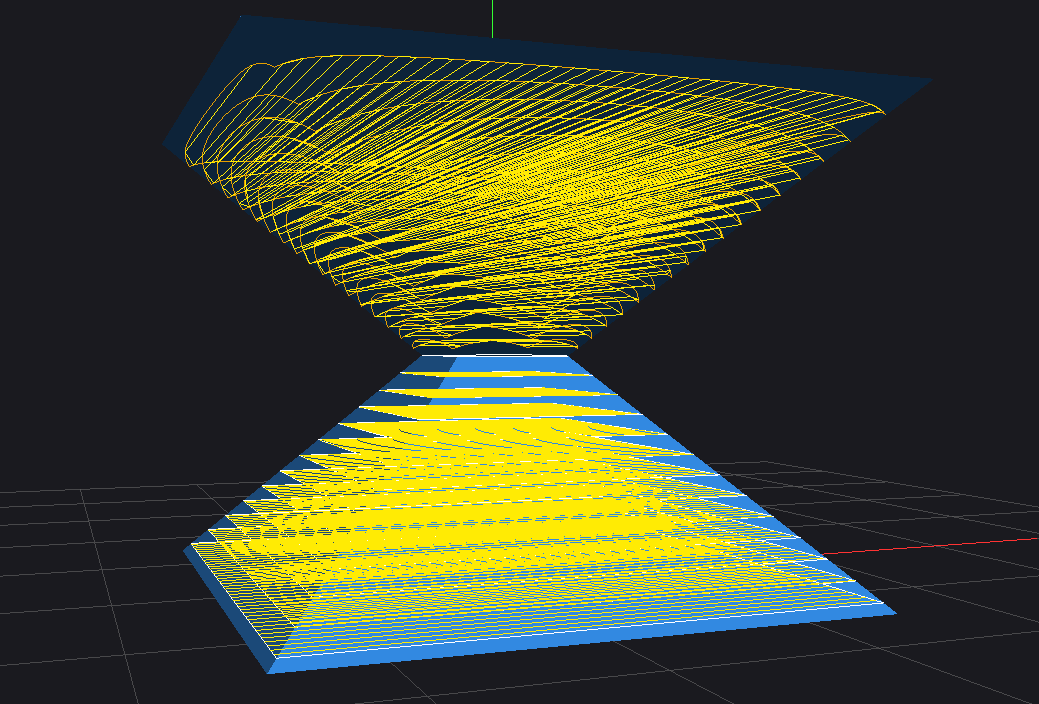
\includegraphics[width=0.4\textwidth]{dependencies/pictures/Pyramide.png}
    \caption{Screenshot der Doppelpyramide in \ac{medusa}, mitsamt der generierten Trajektorien und der Visualisierung des Pathplannings.}
    \label{fig:pyramide}
    \end{figure}


    \begin{figure}[H]
    \centering
    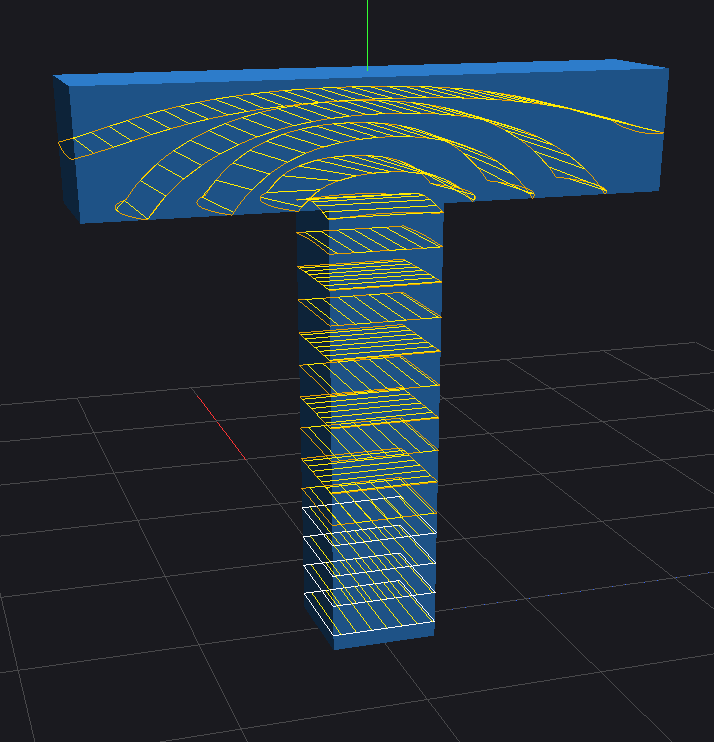
\includegraphics[width=0.4\textwidth]{dependencies/pictures/Tnichtplanar.png}
    \caption{Screenshot des \texttt{T}-Modells in \ac{medusa}, mitsamt der generierten Trajektorien und der Visualisierung des Pathplannings.}
    \label{fig:T-nichtplanar}
    \end{figure}

  \section{Ergebnisse} \label{sec:results}
    Das Ergebnis der vorliegenden Studienarbeit ist ein den Anforderungen aus Abschnitt \ref{subsec:medusa-requirements} entsprechender funktionsfähiger \ac{medusa}-Slicer, welcher die Verarbeitung und Visualisierung von \ac{STL}-Dateien ermöglicht.
    Die Software bietet dem Anwender die Flexibilität, zwischen verschiedenen Ansichtsmodi zu wechseln, um die Geometrie detailliert zu analysieren.

    Wie in Abschnitt \ref{subsec:impl-medusa-slicing-strategies} bereits theoretisch erläutert, verfügt \ac{medusa} über die Fähigkeit, sowohl planare als auch nicht-planare Slicing-Operationen durchzuführen und entsprechende Toolpaths zu generieren.
    Die resultierenden Pfaddaten werden in eine \ac{JSON}-Datei exportiert.
    Im aktuellen Workflow muss diese Datei manuell an das System \ac{kronos} übergeben werden.

    \ac{kronos} übernimmt die Interpretation der \ac{JSON}-Daten und berechnet auf dieser Grundlage die erforderlichen Bewegungsabläufe für den UR3e-Roboterarm.
    Ein wesentlicher Bestandteil von \ac{kronos} ist die integrierte Simulationsumgebung, welche sowohl den Roboterarm als auch das Druckbett realitätsgetreu abbildet.
    Innerhalb dieser Simulation können die berechneten Trajektorien validiert werden, sofern eine kollisionsfreie Pfadfindung erfolgreich war.
    Abschließend bietet das System die Möglichkeit, die verifizierten Bewegungen aus der Simulation direkt auf den physischen Universal Robots UR3e zu übertragen und in der realen Arbeitsumgebung auszuführen.
    \sig{Ben Stahl}

    \subsection{Grenzen und Fehlerszenarien} \label{subsec:limitations-and-failure-scenarios}
      Ein Fehlerfall innerhalb des \ac{kronos}-Systems kann auftreten,
      wenn der Inverse Kinematik Solver für einen vorgegebenen Toolpath keine valide Bewegungslösung berechnen kann.
      Zudem besteht momentan die latente Wahrscheinlichkeit,
      dass die algorithmisch ermittelte Trajektorie keinen rein linearen Pfad darstellt.
      Dies führt dazu, dass der Universal Robots UR3e unvorhersehbare Ausgleichsbewegungen vollzieht,
      welche die Präzision und Sicherheit des Prozesses gefährden könnten.

      Ein weiterer Fehlerzustand im Kontext der \ac{medusa}-Komponente ist zu beobachten,
      sobald die eingelesene \ac{STL}-Datei nicht den strikten Spezifikationen entspricht,
      die in Abschnitt \ref{subsec:medusa-requirements} detailliert definiert wurden.
      Es ist jedoch festzuhalten, dass die automatisierte Korrektur solcher fehlerhaften Dateien
      gemäß der in Abschnitt \ref{subsec:prioritization-and-evaluation-logic} festgelegten Projektziele
      explizit nicht als Bestandteil dieses Vorhabens vorgesehen war.
      \sig{Ben Stahl}

